%% SECTION HEADER /////////////////////////////////////////////////////////////////////////////////////
\section{Results}
\label{sec:resuls}
%% SECTION CONTENT ////////////////////////////////////////////////////////////////////////////////////
\subsection{\acs{hsc} validation with \acs{sldv} setup}
The full wavefield in the reference sample is presented in Fig.~\ref{fig:wavefield}.
The experimental measurements and the \ac{fcgm} snapshots show that the wavefront distortion is rising with the frequency.
Because the wavelength decreases as the frequency increases, a higher frequency signal is more likely to induce wave reflections from the core walls.
This effect is not observed in the case of the \ac{hcgm}.
\begin{figure}[!hbt]
	\begin{center}
		\includegraphics[width=0.95\textwidth]{Chapter_6/fullfield_50_0}
	\end{center}
	\caption{The top surface out of plane particle velocity snapshots for \textbf{(a)} the \acf{fcgm}, \textbf{(b)} the experimental results obtained by using the \acf{sldv}, and \textbf{(c)} the \acf{hcgm} in the \textbf{healthy~sample at 50 kHz}.}
	\label{fig:fullfield_50_0}
\end{figure}
\begin{figure}[!hbt]
	\begin{center}
		\includegraphics[width=0.95\textwidth]{Chapter_6/fullfield_100_0}
	\end{center}
	\caption{The top surface out of plane particle velocity snapshots for \textbf{(a)} the \acf{fcgm}, \textbf{(b)} the experimental results obtained by using the \acf{sldv}, and \textbf{(c)} the \acf{hcgm} in the \textbf{healthy~sample at 100 kHz}.}
	\label{fig:fullfield_100_0}
\end{figure}

\begin{figure}[!hbt]
	\begin{center}
		\includegraphics[width=0.95\textwidth]{Chapter_6/fullfield_150_0}
	\end{center}
	\caption{The top surface out of plane particle velocity snapshots for \textbf{(a)} the \acf{fcgm}, \textbf{(b)} the experimental results obtained by using the \acf{sldv}, and \textbf{(c)} the \acf{hcgm} in the \textbf{healthy~sample at 150 kHz}.}
	\label{fig:fullfield_150_0}
\end{figure}
\begin{figure}[!hbt]
	\begin{center}
		\includegraphics[width=0.95\textwidth]{Chapter_6/fullfield_50_5}
	\end{center}
	\caption{The top surface out of plane particle velocity snapshots for \textbf{(a)} the \acf{fcgm}, \textbf{(b)} the experimental results obtained by using the \acf{sldv}, and \textbf{(c)} the \acf{hcgm} \textbf{with removed core elements at 50 kHz} in damaged area for both numerical models.}
	\label{fig:fullfield_50_5}
\end{figure}

\begin{figure}[!hbt]
	\begin{center}
		\includegraphics[width=0.95\textwidth]{Chapter_6/fullfield_100_5}
	\end{center}
	\caption{The top surface out of plane particle velocity snapshots for \textbf{(a)} the \acf{fcgm}, \textbf{(b)} the experimental results obtained by using the \acf{sldv}, and \textbf{(c)} the \acf{hcgm} \textbf{with removed core elements at 100 kHz} in damaged area for both numerical models.}
	\label{fig:fullfield_100_5}
\end{figure}
\begin{figure}[!hbt]
	\begin{center}
		\includegraphics[width=0.95\textwidth]{Chapter_6/fullfield_150_5}
	\end{center}
	\caption{The top surface out of plane particle velocity snapshots for \textbf{(a)} the \acf{fcgm}, \textbf{(b)} the experimental results obtained by using the \acf{sldv}, and \textbf{(c)} the \acf{hcgm} \textbf{with removed core elements at 150 kHz} in damaged area for both numerical models.}
	\label{fig:fullfield_150_5}
\end{figure}
In case of the damaged sample, the wavefront is not distorted in the damage area bounded by two dotted lines in Fig.~\ref{fig:wavefield_dam5} for all three cases.
Due to the lack of wave leakage into the core, the wave propagates smoothly through the skin.
For the experimental sample and the \ac{fcgm}, interference of waves reflected from the cells and the damage boundary is observed.
The wave interference observed in the \ac{hcgm} refers to waves reflected only from the defect.

\subsection{\acs{hsc} validation with \acsp{pzt} wave acquisition setup}
Validation of the honeycomb structure models and a separate \ac{cfrp} plate intended for the \ac{hsc} sample were done by comparing the group velocity and amplitude of the first packet of \ac{s0} and \ac{a0} arriving at the sensor.
In the Fig.~\ref{fig:signal_exp_raw} are presented examples of the experimentally obtained raw signals for the healthy and damaged samples.
The raw signals are processed for noise reduction and next an envelope of the signals is calculated.
The envelope is used to obtain the amplitude and group velocity of the mods for the model validation and is used in the analytical assessment of damage magnitude.
\begin{figure}[!htb]
	\begin{center}
		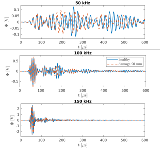
\includegraphics[width=0.95\textwidth]{Chapter_6/signal_exp_raw}
	\end{center}
	\caption{Raw signals registered by the sensor in \acf{hsc} for healthy and damage of 90 \unit{\mm} width.}
	\label{fig:signal_exp_raw}
\end{figure}

Signal processing follows the diagram shown in Fig.~\ref{fig:signal_processing}.
A preliminary step is a conversion of the signals from the time domain to the frequency domain by the \ac{fft}.
Then, the band-pass filter is applied in the range \(0.5f_c-1.5f_c\).
A Butterworth filter of 20th order was used.
After filtering, the signal is again converted to the time domain by the \ac{ifft}.
Lastly, the envelope of the signal \(e(t)\) is obtained using Eq. (\ref{eq:envelope}).

\begin{figure}[!htb]
	\begin{center}
		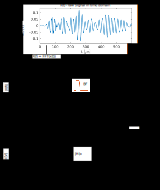
\includegraphics[width=0.95\textwidth]{Chapter_6/signal_processing}
	\end{center}
	\caption{Raw signals registered by the sensor in \acf{hsc} for healthy state and damage of 90 \unit{\mm} width.}
	\label{fig:signal_processing}
\end{figure}

The group velocity is derived from the signal envelope related to particular Lamb wave mode and its \ac{tof}.
The \ac{tof} is a difference between the arrival of the maximum amplitude of the envelope of considered mode at the sensor \((\mathrm{T}_1)\) and the half time of the excitation pulse \(\left(\mathrm{T}_0=\frac{1}{2f_m}\right)\).
Since the distance between the transducers is constant \(l=200\) \unit{\mm}, the group velocity equals:
\begin{eqnarray}
	C_g = \frac{\mathrm{ToF}}{l}=\frac{T_1-T_0}{l}.
\end{eqnarray}

The signal envelopes are shown in Fig.~\ref{fig:single_skin} for single \ac{cfrp} plate, Fig.~\ref{fig:hsc_full} for \ac{fcgm}, and Fig.~\ref{fig:hsc_homo}, from which the velocities and amplitudes of the wave mods were determined.
\begin{figure}[!htb]
	\begin{center}
		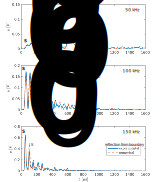
\includegraphics[width=0.95\textwidth]{Chapter_6/single_skin}
	\end{center}
	\caption{The signal envelope for single \acf{cfrp} skin; experimental vs. numerical simulation.}
	\label{fig:single_skin}
\end{figure}
\begin{figure}[!htb]
	\begin{center}
		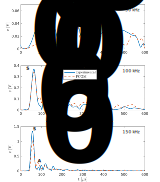
\includegraphics[width=0.95\textwidth]{Chapter_6/HSC_full}
	\end{center}
	\caption{The signal envelope for the \acf{hsc} structure; experimental vs. \acf{fcgm}.}
	\label{fig:hsc_full}
\end{figure}
\begin{figure}[!htb]
	\begin{center}
		\includegraphics[width=0.95\textwidth]{Chapter_6/HSC_homo}
	\end{center}
	\caption{The signal envelope for the \acf{hsc} structure; experimental vs. the \acf{hcgm}.}
	\label{fig:hsc_homo}
\end{figure}

For the single \ac{cfrp} plate, Tab. \ref{tab:group_velocity_cfrp} gives the determined velocities and amplitudes of the modes together with the percentage errors defined by Eq. \ref{eq:perc_err}:
\begin{eqnarray}
	\delta = \left|\frac{x^{num}-x^{exp}}{x^{exp}}\right|\times100\%,
	\label{eq:perc_err}
\end{eqnarray}
\nomtypeG[delta]{\(\delta\)}{Percentage error}{}{\%}%
where \(x^{num}\) and \(x^{exp}\) are the numerical and experimental values, respectively.
It can be noticed that the model are in good agreement with experimental results.
All values are within an error of up to 10\%, except for the \ac{s0} and \ac{a0} amplitudes for 50 and 100 \unit{\kHz}, respectively.
For these cases, the error is about 25\%.
The \ac{a0} mode at 150 \unit{\kHz} in Fig.~\ref{fig:hsc_homo} was not identified because the high amplitude \ac{s0} reflections mask it.

Regarding the \ac{hsc} panel, the best results are achieved for the \ac{fcgm} as it is shown in Tab.~\ref{tab:group_velocity_hsc}.
The velocity error is less than 10\% for both modes except for the signal at 50 \unit{\kHz}. 
In the case of signals amplitude, the simulation results are underestimated.
Only the \ac{s0} at 100 and 150 \unit{\kHz} has the error less than 15\%.
For the \ac{hcgm}, the best result are obtained for the \ac{s0} at 150 \unit{\kHz} with error less than 11\%.
Amplitudes of the \ac{a0} for this model are more accurate than the \ac{fcgm} with the errors below 15\%.

\begin{table}[!htb]
	\small
	\tabcolsep=0.2cm
	\centering
	\caption{\label{tab:group_velocity_cfrp} Comparison between amplitudes and group velocities obtained from the simulations and experiments for the single \acf{cfrp} plate.}
	\begin{tabular}{cccccccc}
		\toprule
		& & \multicolumn{3}{c}{\(C_g\)} & \multicolumn{3}{c}{Amp.}\\
		\multirow{2}{*}{Mode} & Frequency & Exp. & Num. & \(\delta\)& Exp. & Num. & \(\delta\)\\
		& \unit{\kHz} & \unit[per-mode = symbol]{\m\per\s} & \unit[per-mode = symbol]{\m\per\s} & \% & \unit{\mV} & \unit{\mV} & \% \\
		\midrule
		\multirow{3}{*}{\ac{s0}} & 50 & 6079 & 5865 & \textcolor{green}{3.52}& 12 & 171 & \textcolor{red}{25.0} \\
		&100& 5571 & 5747 & \textcolor{green}{3.16} & 171 & 162 & \textcolor{green}{5.26}\\
		&150& 5764 & 5698 & \textcolor{green}{1.15} & 648 & 664 & \textcolor{green}{2.47}\\
		\midrule
		\multirow{3}{*}{\ac{a0}} &50& 1341 & 1325 & \textcolor{green}{0.74} & 134 & 125 & \textcolor{green}{6.72}\\
		&100& 1550 & 1396 & \textcolor{green}{9.74} & 84 & 104 & \textcolor{red}{23.8}\\
		&150& \multicolumn{6}{c}{-} \\
		\bottomrule
	\end{tabular}
\end{table}
\begin{table}[!htb]
	\small
	\tabcolsep=0.15cm
	\centering
	\caption{\label{tab:group_velocity_hsc} Comparison between amplitudes and group velocities obtained from the simulations based on \acf{fcgm} and \acf{hcgm} and experiments for \acf{hsc}.}
	\begin{tabular}{cccccccccccc}
		\toprule
		& & \multicolumn{5}{c}{\(C_g\)} & \multicolumn{5}{c}{Amp.}\\
		\multirow{2}{*}{Mode} & Freq.& Exp. & \ac{fcgm} & \(\delta\) & \ac{hcgm} & \(\delta\) &  Exp. & \ac{fcgm} & \(\delta\) & \ac{hcgm} & \(\delta\)\\
		& \unit{\kHz} & \unit[per-mode = symbol]{\m\per\s} & \unit[per-mode = symbol]{\m\per\s} & \% & \unit[per-mode = symbol]{\m\per\s} & \% & \unit{\mV} & \unit{\mV} & \%& \unit{\mV} & \% \\
		\midrule
		\multirow{3}{*}{\ac{s0}} & 50 & 6452 & 8696 & {34.78} & 8333 & {29.15} & 32 & 6 & \textcolor{red}{81.25} & 3 & \textcolor{red}{90.63}\\
		&100& 5263 & 5128 & \textcolor{green}{2.57} & 5714 & \textcolor{green}{8.57} & 369 & 314 & \textcolor{green}{14.91} & 138 & \textcolor{red}{62.6}\\
		&150& 5085 & 5217 & \textcolor{green}{2.60} & 4959 & \textcolor{green}{2.48} & 1341 & 1239 & \textcolor{green}{7.61} & 1482 & \textcolor{green}{10.51}\\
		\midrule
		\multirow{3}{*}{\ac{a0}} & 50 & 966 & 926 & \textcolor{green}{4.14} & 1316 & {36.23} & 62 & 76 & {22.58} & 63 & \textcolor{green}{1.61}\\
		& 100 & 2174 & 2151 & \textcolor{green}{1.06} & 2273 & \textcolor{green}{4.55} & 137 & 179 & {30.66} & 117 & \textcolor{green}{14.60}\\
		& 150 & \multicolumn{10}{c}{-}\\
		\bottomrule
	\end{tabular}
\end{table}
Errors in the models may be due to several factors.
The most important ones include differences in material properties of used components.
In the models, an average thickness of the adhesive layer was assumed; obtaining precise thickness of the adhesive layer in the specimen preparation is difficult under workshop conditions.
The models also assume a uniform cell geometry for the core area, but in reality, the core is deformed in the plane, so the cell geometry varies.
The velocity in the panel varies with the angle of propagation due to anisotropy of \ac{cfrp} plate and the geometry of the honeycomb core.
In the models, the direction of wave propagation between the sensors was assumed to coincide with the skin and core orientation.
The speed is also affected by the accuracy of the \ac{pzt} placement.